\documentclass{../../../oss-handout}
\usepackage{amsmath,bm}
\usepackage{txfonts}  % must be loaded after amsmath?
\usepackage{enumitem}
\usepackage{tikz}
\usepackage{siunitx}
\usepackage{wrapfig}
%\usepackage{graphicx}
%\usepackage{mathpazo}
%\usepackage{xcolor,colortbl}
%\usepackage{hyperref}
%\usepackage{cancel}

\sisetup{
  detect-all,
  per-mode=symbol
}
%\usetikzlibrary{decorations.pathmorphing,patterns}

\setlength{\parindent}{0pt}
\setlength{\parskip}{8pt}
\setlength{\headheight}{26pt}

\newcommand{\mb}[1]{\ensuremath\mathbf{#1}}
\newcommand{\pic}[2]{\includegraphics[width=#1\textwidth]{#2}}
%\newcommand\vertarrowbox[2]{%
%    \begin{array}[t]{@{}c@{}} #1 \\
%    \rotatebox{90}{$\xrightarrow{\hphantom{abcdefgh}}$} \\[-1ex]
%    \mathclap{\scriptstyle\text{#2}}%
%    \end{array}}


% Set the page style for the document
\pagestyle{plain}

% Course & handout information
\renewcommand{\institution}{Olympiads School, Toronto, ON, Canada}
\renewcommand{\coursetitle}{Advanced Placement Physics (C)}
\renewcommand{\term}{Summer 2020}

\title{Topic 1: Kinematics of Rectilinear Motion}
\author{Dr.\ Timothy Leung}
\date{\today}

\begin{document}
\thispagestyle{title}
\gentitle

\textbf{Kinematics} is a discipline with in mechanics for describing the
motion of points, bodies (objects), and systems of  bodies (groups of objects).
It is the mathematical representation of the relationship between
\emph{position}, \emph{displacement}, \emph{distance}, \emph{velocity},
\emph{speed} and \emph{acceleration}. Note that kinematics does \emph{not}
deal with what causes motion. In high-school level\footnote{Grades 11 and 12 in
  the provincial curriculum} physics courses, kinematics problem usually deals
with motion under constant acceleration. However, in the AP Physics C, we need
a fuller understanding using calculus.

\section{Position}

\begin{wrapfigure}{r}{.35\textwidth}
  \centering
  \vspace{-.1in}
  \begin{tikzpicture}[scale=.5]
    \draw[->](0,0)--(6,0) node[pos=1,right]{$x$};
    \draw[->](0,0)--(0,8) node[pos=1,above]{$y$};
    \draw[->,red,very thick] (0,0)--(4,1) node[midway,above]{$\mb{x}_i$};
    \draw[->,red,very thick] (0,0)--(2,6) node[midway,left]{$\mb{x}_f$};
    \draw[->,blue,very thick](4,1)--(2,6) node[midway,right]{$\Delta\mb{x}$};
    \draw[thick,dash dot,<->] (4,1)..controls (6,5) and (5,7)..(2,6)
    node[midway,right]{$s$};
  \end{tikzpicture}
  \caption{Position, displacement and distance in a Cartesian coordinate
    system.}
  \label{fig:d-vs-d}
\end{wrapfigure}
\textbf{Position} is a vector describing the location of an object in a
coordinate system. For rectinlinear motion, the preferred coordinate system
is the \emph{cartesian} system.\footnote{For circular motions, we will use
  the \emph{polar coordinate system} in 2D, or
  \emph{cylindrical coordinate system} or \emph{spherical coordinate system} in
  3D}. The origin of the coordinate system is called ``reference point''.  In
the IJK notation for rectilinear motion, we can express position of an object
by its $x$, $y$ and $z$ components (i.e.\ their $(x,y,z)$ coordinates). The SI
unit for position is \emph{meters} (\si{\metre}).
\begin{equation*}
  \mb{x}(t)=x(t)\bm{\hat{\imath}} + y(t)\bm{\hat{\jmath}} + z(t)\bm{\hat{k}}
\end{equation*}
If the object is in motion, then the position vector is a function of time $t$.

\section{Displacement}

\textbf{Displacement} is the change in position from $\mb{x}_i$ to
$\mb{x}_f$ within the same coordinate system, whenever an object moves.
\begin{equation*}
  \Delta\mb{x}=\mb{x}_f-\mb{x}_i
  =(x_f-x_i)\bm{\hat{\imath}}+
  (y_f-y_i)\bm{\hat{\jmath}}+
  (z_f-z_i)\bm{\hat{k}}
\end{equation*}
It it illustrated in Fig.~\ref{fig:d-vs-d}. Like position (not surprisingly),
the SI unit for displacement is also \emph{meters}. The use of IJK notation
makes vector addition and subtraction less prone to errors. Note that since
``reference point'' is the origin of the coordinate system, i.e.\
$\mb{x}_{\textrm{ref}}=\mb{0}$, any position vector $\mb{x}$ is also its
displacement from the reference point.



\section{Distance}%{Similar to Displacement}

\textbf{Distance} $s$ is a quantity that is \emph{similar} (and related) to
displacement. It is the \emph{length of the path} taken when an object moves
from position $\mb{d}_1$ to position $\mb{d}_2$, as shown in
Fig.~\ref{fig:d-vs-d}. Unlike displacement, however, distance is a scalar
quantity that is always positive: $s\geq 0$, i.e.\ you can never walk a
\emph{negative} distance to the store. Because the path is not always a
straight line, therefore while the magnitude of the displacement vector is also
a scalar, it is not necessarily the same as distance:
\begin{equation*}
  s\geq |\Delta\mb{d}|
\end{equation*}


\section{Instantaneous \& Average Velocity}

\textbf{Velocity} is a quantity used to describe how \emph{fast} an object is
moving. If position $\mb{x}(t)$ is differentiable in time $t$, then its
\textbf{instantaneous velocity} $\mb{v}(t)$ can be found at any time $t$ by
differentiating $\mb{x}$ with respect to $t$. The SI unit for velocity is
\emph{meters per second} (\si{\metre\per\second}):
% The
%\textbf{instantaneous velocity} of an object is the rate of change of its
%position vector with respect to time:
\begin{equation}
  \boxed{\mb{v}(t)= \frac{d\mb{x}(t)}{dt}}
\end{equation}
Since position $\mb{x}(t)$ has $x(t)$, $y(t)$ and $z(t)$ components along the
(linearly independent) $\bm{\hat{\imath}}$, $\bm{\hat{\jmath}}$ and
$\bm{\hat{k}}$ directions, we can take the time derivative of every component
to obtain the velocity components $v_x$, $v_y$ and $v_z$ in those directions:
\begin{equation*}
  \mb{v}(t)= \frac{d\mb{x}}{dt}=
  \frac{dx}{dt}\bm{\hat{\imath}} +
  \frac{dy}{dt}\bm{\hat{\jmath}} + \frac{dz}{dt}\bm{\hat{k}}=
  v_x\bm{\hat{\imath}} + v_y\bm{\hat{\jmath}} + v_z\bm{\hat{k}}
\end{equation*}
By the fundamental theorem of calculus, if instantaneous velocity $\mb{v}(t)$
is the time derivative of position $\mb{x}(t)$ with respect to time $t$, then
$\mb{x}(t)$ is the time integral of $\mb{v}(t)$:
\begin{equation}
  \boxed{\mb{x}(t)=\int\mb{v}(t)dt + \mb{x}_0}
\end{equation}
The constant of integration $\mb{x}_0=\mb{x}(0)$ is the object's
\emph{initial position} at $t=0$. As was the case in differentiation,
%As both $\mb{x}$ and $\mb{v}$ are vectors,
we can integrate each component to get $\mb{x}$:
\begin{equation*}
  \mb{x}(t)= \left(
  \int v_x\bm{\hat{\imath}} + \int v_y\bm{\hat{\jmath}} + \int v_z\bm{\hat{k}}
  \right) dt + \mb{x}_0
\end{equation*}


The \textbf{average velocity} ($\overline{\mb{v}}$)\footnote{For
  \emph{time averages}, the convention amongst \emph{most} physicists is to
  write a bar over the quantity, as we have done here. In contrast, for
  \emph{ensemble averages}, e.g.\ the average speeds of many particles, we use
  the notation $\big\langle v\big\rangle$. (See thermodynamics slides later in
  the course)} of an object is the change in position $\Delta\mb{x}$ over a
finite time interval $\Delta t$:
\begin{equation}
  \boxed{\overline{\mb{v}}= \frac{\Delta\mb{x}}{\Delta t}}
\end{equation}
Like instantaneous velocity, we can find the $x$, $y$ and $z$ components of
average velocity by separating components in each direction:
\begin{equation*}
  \overline{\mb{v}}=
  \frac{\Delta x}{\Delta t}\bm{\hat{\imath}} +
  \frac{\Delta y}{\Delta t}\bm{\hat{\jmath}} +
  \frac{\Delta z}{\Delta t}\bm{\hat{k}} =
  \overline{v}_x\bm{\hat{\imath}} +
  \overline{v}_y\bm{\hat{\jmath}} +
  \overline{v}_z\bm{\hat{k}}
\end{equation*}



\section{Instantaneous \& Average Speed}

\textbf{Instantaneous speed} $v(t)$ is the rate of change of distance with
respect to time.\footnote{It is regrettable that both velocity and speed use
  the symbol $v$, but \emph{c'est la vie}.} Like velocity, the unit for
speed is also \si{\metre\per\second}:
\begin{equation*}
  \boxed{v(t)=\frac{ds}{dt}}
\end{equation*}
Since distance is a scalar quantity, so too is speed. As distance of any path
must always be positive $s>0$, instantaneous speed must also be positive.
Instantaneous speed $v$ is the magnitude of the instantaneous velocity vector
$\mb{v}$. Likewise, \textbf{average speed} ($\overline{v}$) is similar to
average velocity: it is the distance travelled over a finite time
interval.\footnote{It should be obvious that unlike instantaneous speed, average
  speed is not the magnitude of the average velocity.}
\begin{equation}
  \boxed{\overline{v}=\frac{s}{\Delta t}}
\end{equation}



%\section{Path}
%
%Sometimes instead of explicitly describing the position $x=x(t)$ and $y=y(t)$,
%the path of an object can be given in terms of $x$ coordinate $y=y(x)$, while
%giving the $x$ (or $y$) coordinate as a function of time.
%\begin{itemize}
%\item In this case, substitute the expression for $x(t)$ into $y=y(x)$ to
%  get an expression of $y=y(t)$
%\item Take derivative using chain rule to get $v_y=v_y(t)$
%\end{itemize}


\section{Instantaneous and Average Acceleration}

In the same way that velocity is the rate of change in position with respect
to time, \textbf{instantaneous acceleration} $\mb{a}(t)$ is the rate of change
in velocity with respect to time, and the second time derivative of position.
The SI unit for acceleration is \emph{meters per second squared}
\si{\metre\per\second^2}:
\begin{equation}
  \boxed{\mb{a}(t)= \frac{d\mb{v}(t)}{dt}=\frac{d^2\mb{x}(t)}{dt^2}}
\end{equation}
Although in Grades 11 and 12, students deal almost exclusively with constant
acceleration, in AP Physics, it must be understood that acceleration can also
vary with time, and that calculus must be used in many cases.
%  \begin{enumerate}
%  \item Take derivative of $\mb{x}(t)$ to get $\mb{v}(t)=\mb{x}'(t)$
%  \item Take derivative again of $\mb{v}(t)$ to get $\mb{a}(t)=\mb{v}'(t)$
%  \end{enumerate}
%\end{frame}
Again, by the fundamental theorem of calculus, instantaneous velocity
$\mb{v}(t)$ is the time integral of instantaneous acceleration $\mb{a}(t)$:
\begin{equation}
  \boxed{\mb{v}(t)=\int\mb{a}(t)dt+\mb{v}_0} =
    \left(\int a_x\bm{\hat{\imath}} +
    \int a_y\bm{\hat{\jmath}} +
    \int a_z\bm{\hat{k}}\right) dt +\mb{v}_0
\end{equation}
where $\mb{v}_0$ is the initial velocity at $t=0$.

\section{Expressing Acceleration as Functions of Position and Velocity}

Since, according to Newton's second law of motion, acceleration is related to
the net force, therefore there are instances where acceleration is often
expressed as functions of other motion quantities rather than time. For example:
%for motion that are driven by:
\begin{itemize}[leftmargin=15pt]
\item\textbf{Gravitational force}\footnote{Newton's law of universal
  gravitation: $\displaystyle F_g=\frac{Gm_1m_2}{r^2}$} or
  \textbf{electrostatic force}\footnote{Coulomb's law:
    $\displaystyle F_q=\frac{kq_1q_2}{r^2}$} are both inversely proportional to
  the square of the distance (called the inverse-square law), and acceleration
  is best express by this complicated differential equation:
  \begin{equation*}
    a(x)=\frac{A}{x^2} \quad\text{or}\quad \frac{d^2x}{dt^2}=\frac{A}{x^2}
  \end{equation*}
  The solution will likely require numerical integration.
\item\textbf{Spring force} is proportional to displacement\footnote{By Hooke's
  law $\mb{F}_s=-k\mb{x}$, where $k$ is the spring constant that describes the
  stiffness of the spring}, and acceleration is expressed as:
  \begin{equation*}
    a(x)=-bx\quad\text{or}\quad \frac{d^2x}{dt^2}=-bx
  \end{equation*}
  The solution to this \emph{second-order ordinary differential equation with
    constant coefficient} is a sinusoidal function, i.e.\
  $x(t)=A\sin(\omega t+\phi)$, and the motion is a \emph{simple harmonic
    motion} that will be studied in a later topic.
\item\textbf{Damping force}  is usually proportional to velocity, leading
  to an expression for acceleration
  \begin{equation*}
    a(v)=-cv\quad\text{or}\quad \frac{dv}{dt}=-cv
  \end{equation*}
  This time, the equation is a \emph{first-order ordinary differential equation}
  that can be solved by separating the $dt$ term and $v$ terms and then
  integrating, and the expression for velocity is an exponential function:
  \begin{equation*}
    \frac{dv}{dt}=-cv\quad\rightarrow\quad \int\frac{dv}{v}=-\int cdt
    \quad\rightarrow\quad \ln(v)=-ct+C
    \quad\rightarrow\quad v(t)=v_0e^{-ct}
  \end{equation*}
  Once the velocity expression is obtained, the expression for $x(t)$ and
  $a(t)$ can also easily be obtained by integrating and differentiating.
\item\textbf{Aerodynamic forces} such as drag and lift\footnote{The equations
  for lift and drag forces are $L=\frac12\rho v^2C_LA_\mathrm{ref}$ and
  $D=\frac12\rho v^2C_DA_\mathrm{ref}$ respectively, where $\rho$ is the density
  of the fluid, $A_\mathrm{ref}$ is the reference area, $C_L$ is the lift
  coeffcient and $C_D$ is the drag coefficient}, which are proportional
  to the square of the velocity, leading to an expression for acceleration 
  \begin{equation*}
    a(v)=-kv^2\quad\text{or}\quad \frac{dv}{dt}=-kv^2
  \end{equation*}
  Not surprisingly, the process of solving the problem is similar to that of
  the damping function, but this time, the solution is a hyperbolic function:
  \begin{equation*}
    \frac{dv}{dt}=-kv^2\quad\rightarrow\quad \int\frac{dv}{v^2}=-\int kdt
    \quad\rightarrow\quad -\frac{1}{v}=-kt+C
    \quad\rightarrow\quad v(t)=\frac{1}{ct+C}
  \end{equation*}
\end{itemize}
In practice, multiple forces may act on an object, and each of them will be
functions of other motion quantities, and therefore the solution may require
solving more complex differential equations (although this is highly unlikely in
AP Physics).

\section{Special Notation When Differentiating With Time}

Physicists and engineers often use a special notation when the derivative is
taken with respect to \emph{time} (and not spatial derivatives), by writing a
dot above the variable for \emph{first} derivative, and \emph{two} dots for
\emph{second} derivative, etc. For example, velocity is
$\mb{v}(t)=\dot{\mb{x}}$ while acceleration is
$\mb{a}(t)= \dot{\mb{v}}=\ddot{\mb{x}}$. This notation will be used occasionally
in this course when it is convenient to do so.


\section{Higher Derivatives}

For those who are curious about higher derivatives, the time derivative of
acceleration is called \textbf{jerk} $\mb{j}(t)$ with a unit of
\si{\metre\per\second^3}:
\begin{equation}
  \mb{j}(t)=\frac{d\mb{a}}{dt}=\frac{d^2\mb{v}}{dt^2}=\frac{d^3\mb{x}}{dt^3}
\end{equation}
The measurement of jerk is used in many sensors, for example, in accelerometers
in airbags to determine if the acceleration of a car is under normal operation
(small $j$ value) or if a crash is in progress (high $j$ value). The time
derivative of jerk is \textbf{jounce}, or \textbf{snap}, with unit of
\si{\metre\per\second^4}:
\begin{equation}
  \mb{s}(t)=\frac{d\mb{j}}{dt}=\frac{d^2\mb{a}}{dt^2}=\frac{d^3\mb{v}}{dt^3}
  =\frac{d^4\mb{x}}{dt^4}
\end{equation}
The next two derivatives of snap is facetiously called \textbf{crackle} and
\textbf{pop}\footnote{As in the cartoon mascots for Kellogg's rice crispies},
but these higher derivatives are rarely used, and will \emph{not} be used in
in AP Physics.



\section{Kinematic Equations for Constant Acceleration}

Although kinematic problems in AP Physics often require calculus\footnote{Unlike
  your AP Calculus exams, the differentiation/integration in AP Physics will be
  fairly straightforward}, basic kinematic equations for \emph{constant}
acceleration are still a very powerful tool. For constant acceleration
$\mb{a}$, velocity can be obtained by integrating in time:
\begin{equation}
  \mb{v}(t)=\int\mb{a}dt\quad\rightarrow\quad\boxed{\mb{v}(t)=\mb{v}_0+\mb{a}t}
  \label{eq:big5-1}
\end{equation}
where $\mb{v}_0$ is the initial velocity at $t=0$. Integrating again for the
position vector:
\begin{equation}
  \mb{x}(t)=\int \mb{v}dt\quad\rightarrow\quad
  \boxed{\mb{x}(t)=\mb{x}_0+\mb{v}_0t+\frac12 \mb{a}t^2}
  \label{eq:big5-2}
\end{equation}
where $\mb{x}_0$ is the initial position at $t=0$. The position vector is
quadratic in time.

The derivation of the last equation is slightly more laborious. From
Eqs.~\ref{eq:big5-1} and \ref{eq:big5-2}, if acceleration is constant, then
both the the velocity and position vectors are continuously differentiable. In
a one-dimensional problem\footnote{for simplicity}, the differentiation can be
expressed as:
\begin{align*}
  \frac{dv}{dt}&=\frac{dv}{dx}\frac{dx}{dt}\\
  a&=v\frac{dv}{dx}
\end{align*}
Multiplying both sides by $dx$ and integrating, we have:
\begin{align*}
  \int_{x_0}^x adx&=\int_{v_0}^v vdv\\
  a(x-x_0)&=\frac12\left(v^2-v_0^2\right)
\end{align*}
or in the more familiar form:
\begin{equation}
  \boxed{v^2 = v_0^2+ 2a(x-x_0)}
  \label{eq:big5-3}
\end{equation}
Eqs.~\ref{eq:big5-1}, \ref{eq:big5-2} and \ref{eq:big5-3} are provided in the
AP Exam equation sheet.
%\begin{frame}{Solving Typical Kinematics Problems}
%  
%  \textbf{One object:} the problem provides $3$ of the $5$ variables, and you
%  are asked to find a $4$th one.
%  \begin{itemize}
%  \item Define the positive direction (usually very obvious)
%  \item Apply the correct kinematic equation and solve the problem!
%  \end{itemize}
%
%  \vspace{.2in}\textbf{Two objects:} two objects are in motion. Usually one of
%  them is moving at constant velocity while the other is accelerating.
%  \begin{itemize}
%  \item Time interval $\Delta t$ and displacement $\Delta\mb{x}$ of the two
%    objects are related
%  \item Examples:
%    \begin{itemize}
%    \item Police car chasing a speeder
%    \item Two football players running towards each other
%    \item A person trying to catch the bus
%    \end{itemize}
%  \end{itemize}
%\end{frame}



\end{document}
